\documentclass[12pt,a4paper]{article}
\usepackage{enumerate} 	% put in numbers or bullet points
\usepackage{setspace}	% line spacing					
\usepackage{authblk}	% For author affiliations
\usepackage{graphicx} 	% For adding pictures
\usepackage{pdflscape}	% for landscape pages
\usepackage{mathtools}	% For equations etc.
\usepackage[osf]{mathpazo} 
\usepackage{float}		
\floatstyle{plaintop} 	% Force table captions to go above the table
\usepackage{longtable}
\usepackage[margin ={2cm, 2cm, 2cm, 2cm}]{geometry}
\usepackage[round]{natbib}
\usepackage{hyperref} %need this for url references
\usepackage[parfill]{parskip}

\setcounter{secnumdepth}{0} % removes numbers from section headings
\raggedright 			% justify the text on the left only
\pagenumbering{arabic}
\linespread{1.3}
	
%Label tables as S1, S2 etc.	
\newcommand{\beginsupplement}{%
	       \setcounter{table}{0}
	        \renewcommand{\thetable}{S\arabic{table}}%
	        \setcounter{figure}{0}
	        \renewcommand{\thefigure}{S\arabic{figure}}%
	     }
	
\begin{document}
\beginsupplement

{\centering\section{Supplementary Material}}

\subsection{Landmark descriptions}
\vspace*{-0.5cm}
	The information below provides further details about the landmarks we used to summarise morphological shape in tenrec and golden mole skulls. Landmark numbers and curve descriptions refer to Figure 2 in the main paper (example of a tenrec skull) and also Figure S1 (example golden mole skull). One of us (SF) placed all of the landmarks on each picture.
	
	
	\begin{figure}[!htbp]
	\centering
	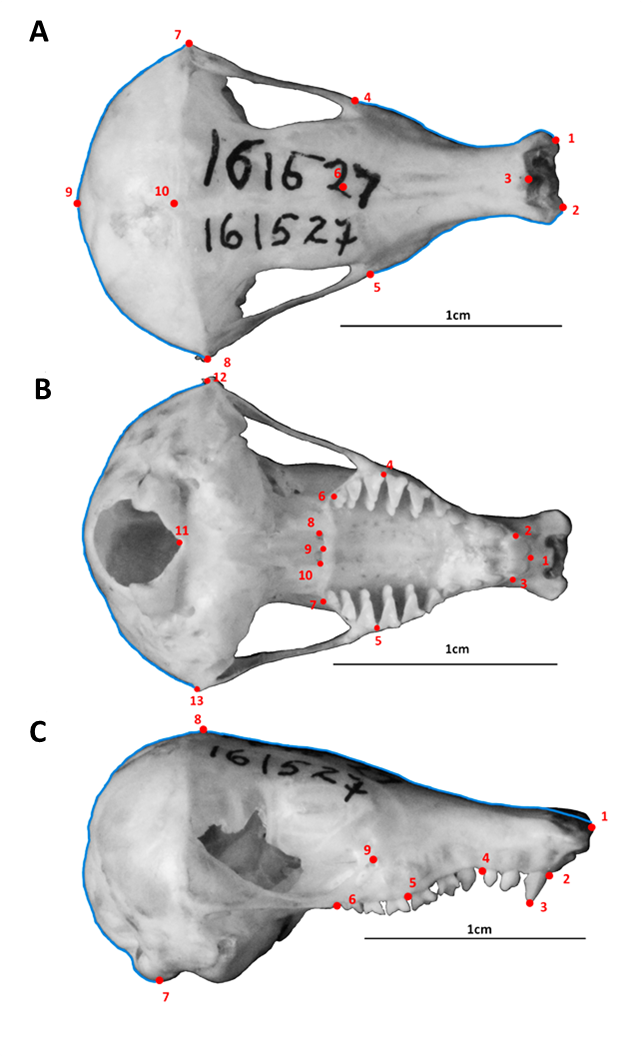
\includegraphics[width=0.8\linewidth, height=0.8\textheight, keepaspectratio]{figures/Gmole_combined_col_light_labels.png}
	\caption[]
		{Landmarks (numbered points) and curves (outlines) for the skulls in dorsal (A), ventral (B) and lateral (C) view. See Tables S1, S2 and S3 for more detailed landmark descriptions. The skulls are an example of a \textit{Chlorotalpa duthieae} (Duthie's golden mole), museum accession number AMNH 161527.}
	\label{fig:gmole}
	\end{figure}

\subsubsection{Skulls: dorsal view}
\vspace*{-0.5cm}
	Most of our landmarks in this view are relative (type 3) points which represent overall morphological shape but not necessarily homologous biological features \citep{Zelditch2012}. We placed ten landmarks and drew four semilandmark curves to represent the shape of both the braincase (posterior) and nasal (anterior) area of the skulls. Table \ref{tab:skdors} describes how we defined the landmarks and outline curves for our images of skulls in dorsal view.

%Table with skdors landmark descriptions
\begin{table}[h]
	\caption[Skulls: dorsal landmarks]
		{Descriptions of the landmarks (points) and curves (semilandmarks) for the skulls in dorsal view} 
	%Skdors landmarks


\begin{tabular}[t]{p{0.2\textwidth} p{0.75\textwidth}}		
\hline
\textbf{Landmark} & \textbf{Description} \\
\hline
%------------------------------------------------------------
1 + 2 & Left (1) and right (2) anterior points of the premaxilla \\
%------------------------------------------------------------
3 & Anterior of the nasal bones in the midline \\
%------------------------------------------------------------
4 + 5 &	Maximum width of the palate (maxillary) on the left (4) and right (5)\\
%------------------------------------------------------------
6 & Midline intersection between nasal and frontal bones \\
%------------------------------------------------------------
7 + 8 & Widest point of the skull on the left (7) and right (8) \\
%------------------------------------------------------------
9 &	Posterior of the skull in the midline \\
	%Panchetti 2008 and Macholan2008 have different definitions for this one so I need to choose one
%------------------------------------------------------------
10 & Posterior intersection between saggital and parietal sutures \\
%--------------------------------------
\hline
Curve A (12 points) & Outline of the braincase on the left side, between landmarks 7 and 9 (does not include visible features from the lower (ventral) side of the skull) \\

Curve B (10 points) & Outline of the palate on the left side, between landmarks 1 and 4 (outline of the rostrum only, not the shape of the teeth)\\

Curve C (12 points) &	Outline of the braincase on the right side, between landmarks 8 and 9 (does not include visible features from the lower (ventral) side of the skull) \\

Curve D (10 points) & Outline of the palate on the right side, between landmarks 2 and 5 (outline of the rostrum only, not the shape of the teeth)\\
%------------------------------------------------------------
\hline
\end{tabular}
	\label{tab:skdors}
\end{table}
%--------------------------------------------------------------

\subsubsection{Skulls: ventral view}
\vspace*{-0.5cm}
	Most of the landmarks in this view are concentrated around the dentition and palate of the animals. We identified 13 landmarks and drew one outline curve (resampled to 60 semilandmark points) around the back of the skull between landmarks 12 and 13. The high variability of our species' basi-cranial regions and difficulties associated with identifying developmentally or functionally homologous points precluded designation of additional landmarks towards the back of the skulls. Table \ref{tab:skvent} outlines the descriptions of the landmarks we used for the ventral skull photos.

% Skulls ventral landmarks
\begin{table}[!htb] 
\caption[Skulls: ventral landmarks]
		{Descriptions of the landmarks (points) and curves (semilandmarks) for the skulls in ventral view.} 
%SkVent landmarks
\begin{tabular}[t]{p{0.2\textwidth} p{0.75\textwidth}}		
\hline
\textbf{Landmark} & \textbf{Description} \\
\hline
%--------------------------------------
1 & Anterior point of the palate\\
%--------------------------------------
2 + 3 & Posterior, lateral extremity of the right (2) and left (3) incisor\\
%--------------------------------------
4 + 5 & Anterior, outer point of the first molar on the right (4) and left (5)\\
%--------------------------------------
6 + 7 & Posterior, outermost point of the last molar surface on the right (6) and left (7) \\
%--------------------------------------
8 & Widest point of the curve of the palatine on the right side\\
%--------------------------------------
9 & Posterior point of the palatine in the midline\\
%--------------------------------------
10 & Widest point of the curve of the palatine on the left side\\
%--------------------------------------
11 & Anterior of the occipital foramen in the midline\\
%--------------------------------------
12 + 13 & Widest (extreme lateral) point of the braincase on the right (12) and left (13)\\
%--------------------------------------
Curve*  & Outline of the back of the skull (between landmarks 12 and 13), 60 points \\
%------------------------------------------------------------
\hline
\end{tabular}
\label{tab:skvent}
\\
*This curve does not necessarily trace homologous features because of the variation in the position of the foramen magnum.
\end{table}
	
%------------------------------------------------------
\newpage
\subsubsection{Skulls: lateral view}
\vspace*{-0.5cm}
	We placed nine landmarks on the photographs of skulls in lateral view and also drew two semilandmark curves to represent the shape of the back of the skull (between landmarks 7 and 8, re-sampled to 20 semilandmark points) and the top of the skull (between landmarks 8 and 1, re-sampled to 15 semilandmark points). Table \ref{tab:sklat} describes our definitions for each of the landmark points.
	If specimens were damaged on their right side we reflected photographs of the left lateral side of the skull so that all the images were in the same orientation.

% Skulls lateral landmarks
\begin{table}[!htb]
\caption[Skulls: lateral landmarks]
		{Descriptions of the landmarks (points) and curves (semilandmarks) for the skulls in lateral view.} 
%Sklat landmarks

\begin{tabular}[t]{p{0.2\textwidth} p{0.75\textwidth}}		
\hline
\textbf{Landmark} & \textbf{Description} \\
\hline
%--------------------------------------
1 & Anterior, upper tip of the nasal bone\\
%--------------------------------------
2 & Anterior of the alveolus of the first incisor\\
%--------------------------------------
3 & Lowest point of the first incisor\\
%--------------------------------------
4& Posterior of the alveolus of the last incisor \\
%--------------------------------------
5 & Anterior tip of the alveolus of the first molar\\
%--------------------------------------
6 & Posterior tip of the alveolus of the last molar\\
%--------------------------------------
7 & Lowest point of the basi-occipital (base of the back of the skull)\\
%--------------------------------------
8 & Highest point of the braincase\\
%--------------------------------------
9 & Highest point of the infraorbital foramen\\
%--------------------------------------
\hline
Curve A & Between points 7 and 8  \\
(20 points)& Back of the skull from the lowest to highest points\\
%------------------------------------------------------------
Curve B & Between points 8 and 1  \\
(15 points)&From the highest point of the braincase to the front of the nasal \\
%------------------------------------------------------------
\hline
\end{tabular}
\label{tab:sklat}
\end{table}
%-------------------------------------------
\subsection{{Potential morphometrics errors}}
\vspace*{-0.5cm}	 
	While 2D methods are an accepted means of comparing morphological shape \citep[e.g.][]{Adams2004, Mitteroecker2009}, particularly for comparing skull morphologies of small mammals \citep[e.g.][]{Cardini2003, Panchetti2008, White2008, Barrow2008, Scalici2011}, the inherent discrepancies associated with comparing three dimensional objects using two dimensional pictures can introduce some potential problems of possible image distortion \citep{Arnqvist1998}. Similarly, human error with how landmarks are positioned on specimens could also introduce noise into further analyses.
	In contrast to detailed intraspecific work \citep[e.g.][]{Bornholdt2008, Blagojevic2011}, photographic or landmark placement errors are unlikely to be significant in our interspecific study since one would expect that the morphological variation among species is large enough to  be detected as a signal above any background noise associated with methodological error \citep{Arnqvist1998}. Nevertheless, it is still important to assess measurement error in a morphometric data set to increase confidence in the outcome of final analyses.
	We identified two possible sources of morphometric measurement error: specimen orientation and placement of landmarks.

    Variation in the orientation of specimens for photography is one of the main sources of error in 2D morphometric studies \citep{Adriaens2007}. If specimens are not placed on a flat plane or in a consistent position relative to the camera, areas of the object which are tilted towards the camera will appear to be larger than in reality, distorting any subsequent morphometric analyses of the shape. 
	One of us (SF) placed the landmarks on each set of pictures so inter-observer variation in landmark placement is not an issue for our study.  However, repeatability and reliability of our choice of landmarks could affect the final results of the analyses \citep{Arnqvist1998}.

	
	To measure potential orientation error, we photographed the skulls (dorsal, ventral and lateral views) of each specimen three times, cycling through the photos so that the specimen was removed and re-positioned before every shot \citep{Viscosi2011}.
	We used a subset of the ventral skull images to test for two sources of error: specimen orientation and landmark placement error \citep{Arnqvist1998, Barrow2008}. Of the specimens which we photographed three times, we chose a random subset of seven skulls from four different Families: three tenrecs and single representatives of shrews, moles, hedgehogs and golden moles. We copied these images and placed landmarks on three copies of each image to compare variation in landmark placement within each orientation. This gave nine replicates of each skull: three separate photos, and three copies of each of those photos. As before, we ran a general Procrustes alignment \citep{Rohlf1993} of the specimens, calculated the average shape values for each skull (average of all nine pictures) and used these values for a principal components (PC) analysis.
		
	We used a linear mixed effects model to model the shape variation (first PC axis) associated with specimen (fixed effect) and two nested random effects: photo identity nested within specimen and image replicate nested within each photograph. This nested approach was necessary to deal with the hierarchical nature of our data subset: three photos of every specimen and three replicates of each of those images. We ran the test using the lmer function in the lme4 package \citep{Bates2014}.  

	We found that specimen orientation and landmark placement have negligible effects on the overall shape variation between different skulls: the random effect variables of photo identify and image replicate explained less than 0.0001 \% of the overall shape variation among different skulls. Therefore, we are confident that shape variation among the specimens in the rest of the analyses reflects true morphological differences rather than methodological error.
%---------------------------------------
\section{Sample size}


The total number of photographs used for each analysis differed slightly because some skull specimens were damaged and could only be used for certain views (see main text). Table \ref{tab:samp} summarises the total number of specimens used for each of the three analyses. We accounted for differences in sample size by analysing the average skull shape of each species and using permutation tests to ensure that differences in relative morphological diversity were not artefacts of differences in overall group size (see main text).

\begin{table}[!htbp] 
\caption[Sample size]
		{Summary of the sample size (number of skull specimens) used for each analysis: skulls in dorsal, ventral and lateral view.} 
%Sample size of specimens for each analysis

%\resizebox{\columnwidth}{!}{
\begin{tabular}[t]{l l c c c}		
\hline
%------------------------------------------
Family & Species & \multicolumn{3}{c}{Number of Specimens}\\
%-------------------
\cline{3-5}
%-------------------------------------------
 &  & Dorsal & Ventral & Lateral\\
%-----------------------------------------
\hline
Chrysochloridae & \textit{Amblysomus corriae} & 1 & 1 & 1\\
%-------------------------------------------
Chrysochloridae & \textit{Amblysomus hottentotus} & 4 & 4 & 4 \\
%-------------------------------------------
Chrysochloridae & \textit{Calcochloris leucorhinus} & 3 & 3 & 3 \\
%-------------------------------------------
Chrysochloridae & \textit{Calcochloris obtusirostris} & 4 & 3 & 2 \\
%-------------------------------------
Chrysochloridae & \textit{Carpitalpa arendsi} & 1 & 1 & 1\\
%-------------------------------------------
%----------------------------------
Chrysochloridae & \textit{Chlorotalpa duthieae} & 3 & 2 & 3\\
%-------------------------------------------
Chrysochloridae & \textit{Chrysochloris asiatica} & 4 & 4 & 3 \\
%-------------------------------------------
Chrysochloridae & \textit{Chrysochloris stuhlmanni} & 4 & 4 & 4 \\
%-------------------------------------------
Chrysochloridae & \textit{Chrysospalax trevelyani} & 4 & 4 & 4 \\
%-------------------------------------------
Chrysochloridae & \textit{Chrysospalax villosus} & 1 & 1 & 1\\
%-------------------------------------------
Chrysochloridae & \textit{Cryptochloris wintoni} & 2 & 2 & 2\\
Chrysochloridae & \textit{Eremitalpa granti} & 3 & 3 & 3\\
%-------------------------------------------
%Tenrecs
%-------------------------------------------
Tenrecidae & \textit{Echinops telfairi} & 5 & 5 & 5\\
%-------------------------------------------
Tenrecidae & \textit{Geogale aurita} & 5 & 4 & 5\\
%-------------------------------------------
Tenrecidae & \textit{Hemicentetes nigriceps} & 5 & 4 & 4\\
%-------------------------------------------
Tenrecidae & \textit{Hemicentetes semispinosus} & 6 & 5 & 5 \\
%-------------------------------------------
Tenrecidae & \textit{Limnogale mergulus} & 1 & 1 & 1\\
%-------------------------------------------
Tenrecidae & \textit{Microgale brevicaudata} & 5 & 5 & 5 \\
%-------------------------------------------
Tenrecidae & \textit{Microgale cowani} & 6 & 6 & 6\\
%-------------------------------------------
Tenrecidae & \textit{Microgale dobsoni} & 5 & 4 & 5\\
%-------------------------------------------
Tenrecidae & \textit{Microgale drouhardi} & 5 & 5 & 5 \\
%-------------------------------------------
Tenrecidae & \textit{Microgale dryas} & 5 & 5 & 4\\
%-------------------------------------------
Tenrecidae & \textit{Microgale fotsifotsy} & 5 & 5 & 5 \\
%-------------------------------------------
Tenrecidae & \textit{Microgale gracilis} & 5 & 5 & 4\\
%-------------------------------------------
Tenrecidae & \textit{Microgale grandidieri} & 5 & 5 & 5\\
%-------------------------------------------
Tenrecidae & \textit{Microgale gymnorhyncha} & 5 & 5 & 5 \\
%-------------------------------------------
Tenrecidae & \textit{Microgale jobihely} & 5 & 5 & 5\\
%-------------------------------------------
Tenrecidae & \textit{Microgale longicaudata} & 5 & 5 & 5 \\
%-------------------------------------------
Tenrecidae & \textit{Microgale monticola} & 5 & 5 & 5 \\
%-------------------------------------------
Tenrecidae & \textit{Microgale parvula} & 4 & 4 & 5\\
%-------------------------------------------
Tenrecidae & \textit{Microgale principula} & 5 & 5 & 5\\
%-------------------------------------------
Tenrecidae & \textit{Microgale pusilla} & 5 & 5 & 5\\
%-------------------------------------------
Tenrecidae & \textit{Microgale soricoides} & 5 & 4 & 4\\
%-------------------------------------------
Tenrecidae & \textit{Microgale taiva} & 5 & 5 & 4 \\
%-------------------------------------------
Tenrecidae & \textit{Microgale talazaci} & 5 & 5 & 5\\
%-------------------------------------------
Tenrecidae & \textit{Microgale thomasi} & 5 & 5 & 5\\
%-------------------------------------------
Tenrecidae & \textit{Micropotamogale lamottei} & 2 & 2 & 2\\
%-------------------------------------------
Tenrecidae & \textit{Micropotamogale ruwenzorii} & 1 & 1 & 1\\
%-------------------------------------------
Tenrecidae & \textit{Oryzorictes hova} & 5 & 5 & 5 \\
%-------------------------------------------
Tenrecidae & \textit{Oryzorictes tetradactylus} & 6 & 6 & 6\\
%-------------------------------------------
Tenrecidae & \textit{Potamogale velox} & 6 & 6 & 5\\
%-------------------------------------------
Tenrecidae & \textit{Setifer setosus} & 5 & 4 & 3\\
%-------------------------------------------
Tenrecidae & \textit{Tenrec ecaudatus} & 6 & 5 & 6\\
%------------------------------------------------------------
\hline
\end{tabular}

\label{tab:samp}
\end{table}
\newpage
\bibliographystyle{sysbio} 
\bibliography{refs_paper} 
\end{document}